\documentclass{article} % For LaTeX2e
\usepackage[T1]{fontenc}
\usepackage[utf8]{inputenc}
\usepackage{lmodern}
\usepackage{fullpage}
\usepackage{amsmath}
\newcommand{\tab}{\hspace*{2em}}
\usepackage{times}
\usepackage{natbib}
\usepackage{algorithm}
\usepackage{algorithmic}
\usepackage{amsmath}
\usepackage{amsthm}
\usepackage{amsfonts}
\usepackage{amssymb}
\usepackage{multirow}
\usepackage{geometry}
\usepackage[pdftex]{graphicx}     
 \graphicspath{{../pdf/}{../jpeg/}{./image/}}  
\title{\Large{\textbf{ Implementation  Assignment 3: Kmeans clustering }}}

\author{
Amir Azarbakht, Mandana Hamidi\\
\small School of Electrical Engineering \& Computer Science\\ 
\small Oregon State University\\
\small 1148 Kelley Engineering Center\\
\small Corvallis, OR 97331\\
\small\texttt{\{azarbaam,hamidim\}@eecs.oregonstate.edu}
}
\date{}
\begin{document}
\maketitle


\begin{abstract}
`The main objective of this assignment is to implement $Kmeans$ clustering algorithm. We did three different experiments for implementing clustering algorithm: first, we implemented the $Kmeans$ with randomly initialized cluster centers. Second, we implemented an algorithm for finding the best number of clusters. In the last part of the assignment we analyze the effect of the feature normalization on the performance of the the $Kmeans$ algorithm.
\end{abstract}

\section{K means Initialization }
In this section, we implemented  a $Kmeans$ algorithm with $k = 5$ on the provided $data1$ with randomly initialized cluster centers for $200$ times. Each time, initially, we randomly picked five unique points in the data to serve as the initial centers and ran $kmeans$ algorithm to convergence. We repeated this for $200$ times and recorded the centers that were found.\\
$Figure~\ref{fig:fig_Kmeans_with_random_initialization}$  represents the recorded cluster centers over $200$ runs, the original data points are plotted in blue color and the found cluster centers in the $200$ runs in cyan color.\\

\begin{figure}[h]
\begin{center}
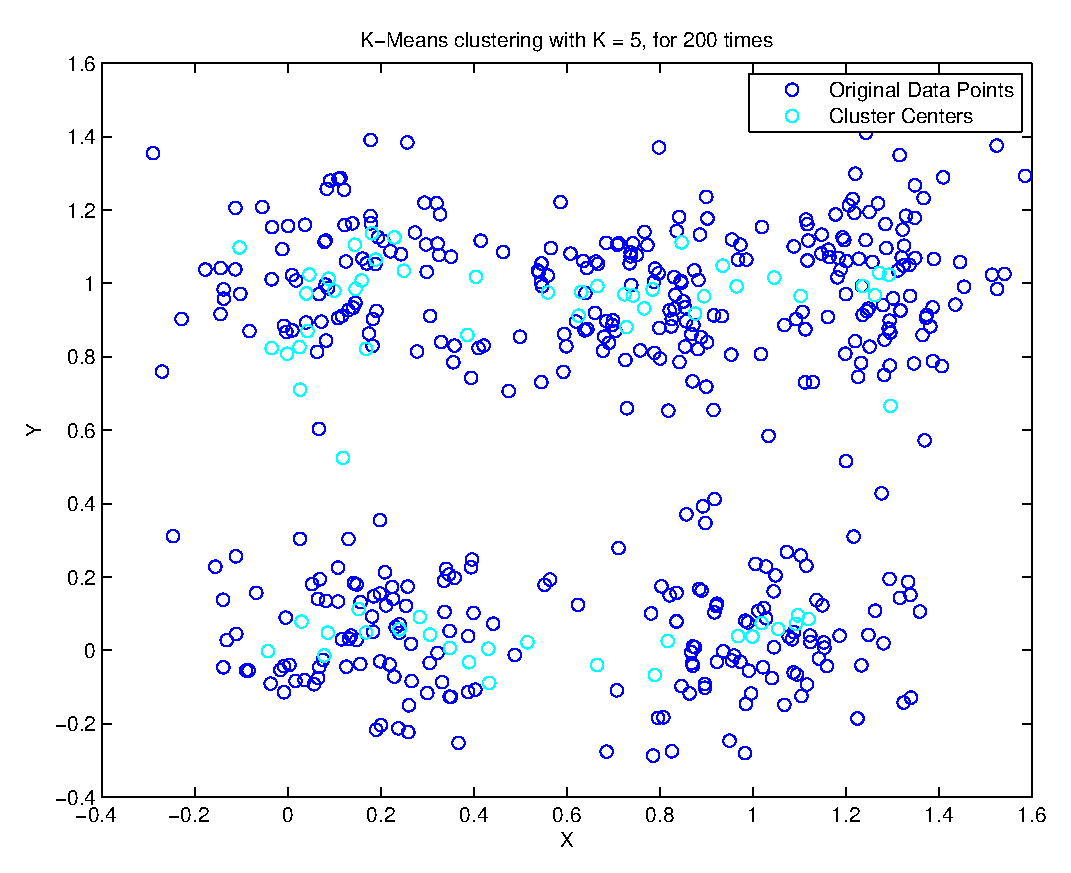
\includegraphics[width=11cm]{Fig/fig_Kmeans_with_random_initialization.eps}
\end{center}
\caption{\small{$Kmeans$ clustering results over 200 runs.The original data points are represented in blue color and the found cluster centers are represented in cyan color}}
\label{fig:fig_Kmeans_with_random_initialization}
\end{figure}

$Table~\ref{table:MinMaxMeanSTD}$ shows the values for minimum, maximum, average, and standard deviation of within-cluster sum or squared distances for the clustering found by our algorithm in the 200 random runs.

\begin{table}[H]
\begin{center}
\centering
\caption{\small{Minimum, Maximum, Average and Standard Deviation of within-cluster sum or squared distances for the clustering found by our algorithm in the 200 random runs}}
\begin{tabular}{|r|r|r|r|}
\hline
Min & Max & Mean & Standard Deviation \\\hline
23.0235&54.3563&25.9688&5.2813\\\hline
\end{tabular}
\end{center}
\label{table:MinMaxMeanSTD}
\end{table}

%\begin{figure}[h]
%\begin{center}
%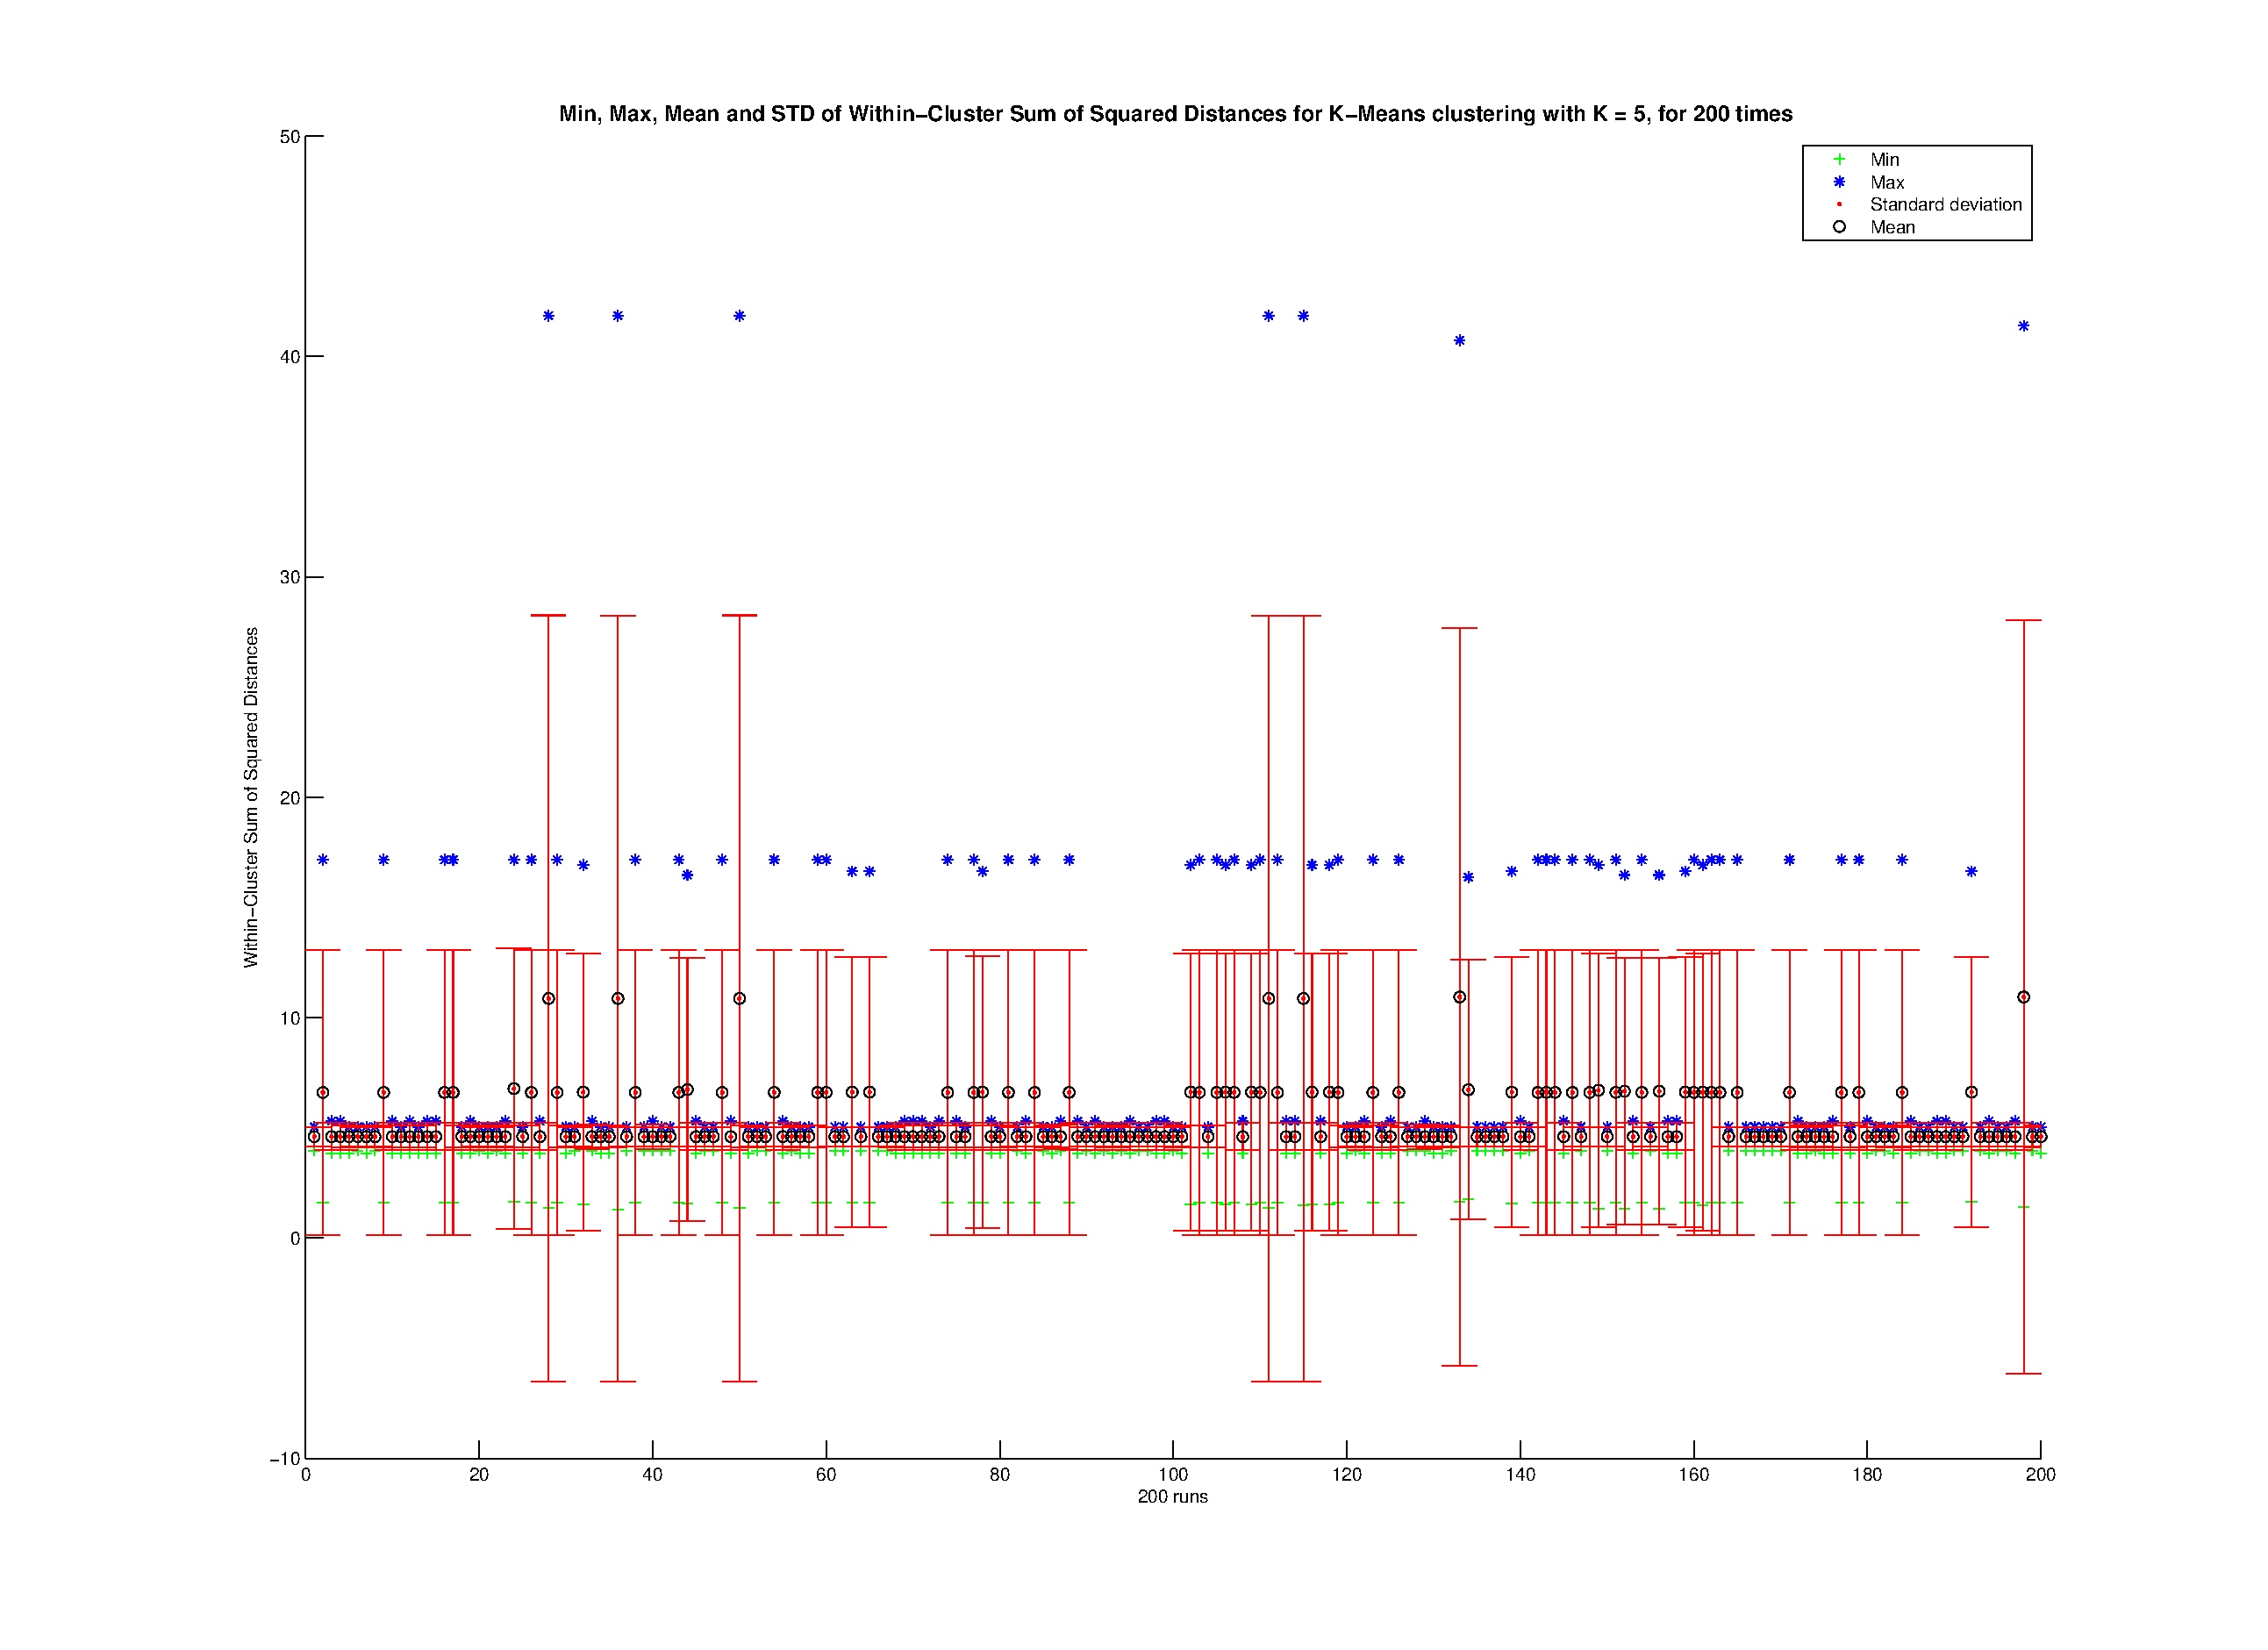
\includegraphics[width=16cm]{Fig/fig_Within_cluster_sum_of_squared_distances_200runs.eps}
% \end{center}
%% \caption{\small{$within$ Within_cluster_sum_of squared distances results for 200 runs.}} 
%\label{fig:fig_Within_cluster_sum_of_squared_distances_200runs}
%\end{figure}

Our results showed that the K-means algorithm found different cluster centres in different runs, mainly due to the random initialization of the initial cluster centers. This shows that the K-means algorithm is sensitive and not robust with regard to the choice of initial seeds. The best within-cluster sum of squared distances over the 200 runs was achieved to be 23.0235, which was close to the average within-cluster sum of squared distances of 25.9688. The worst within-cluster sum of squared distances over the 200 runs was 54.3563, which was almost twice as much as the mean or minimum, which shows that the algorithm can make a really bad clustering decision because of its sensitivity to its initial seeds. The standard deviation of the within-cluster sum of squared distances over the 200 runs was 5.2813, which is almost a quarter of the mean or minimum values, which shows that the clustering decision learned by our K-means algorithm varies to some extend over 200 random runs, and this variability testifies to the sensitivity of the K-means algorithm to its random seeds.

\section{Finding K }
In this section, our objective was to find the best number of clusters using the K-means algorithm. We considered a variety of different k values $\left(k = 2, 3, ..., 15\right)$ and for each k value, we ran our K-means algorithm with 10 different random initializations and recorded the lowest within-cluster sum of squared distances obtained for that $k$ value. 

\begin{figure}[h]
\begin{center}
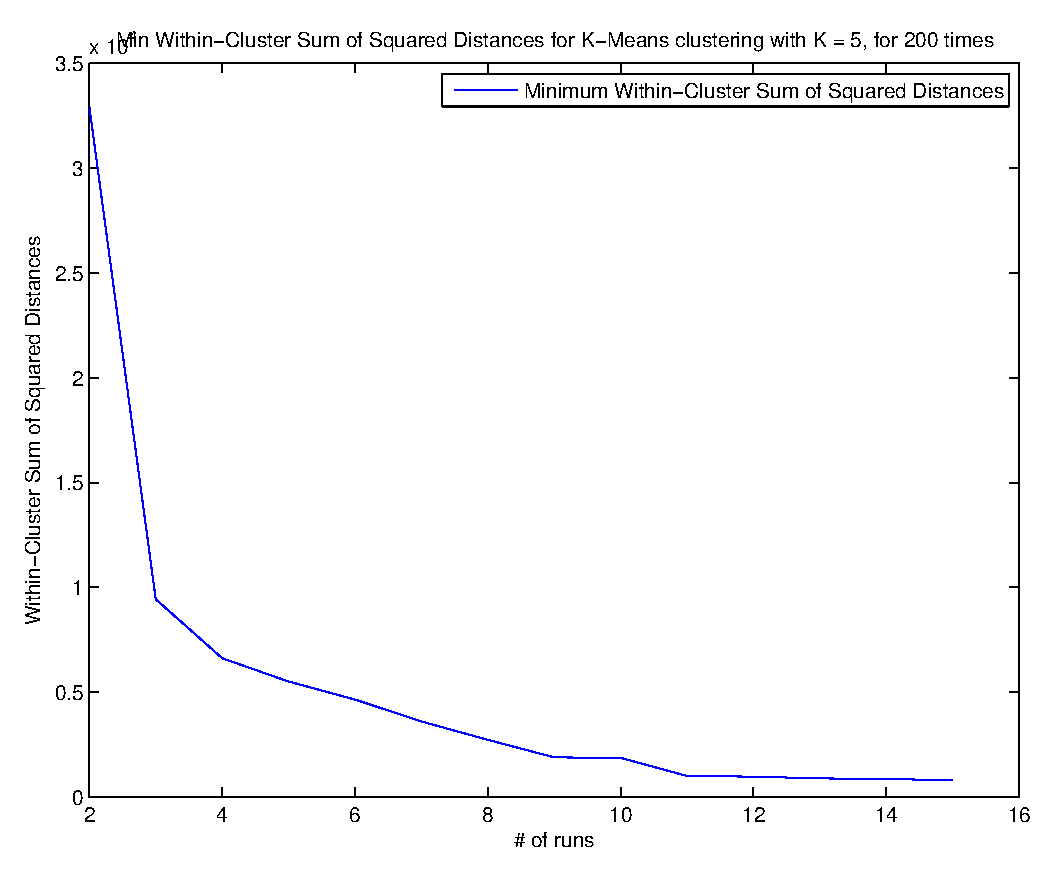
\includegraphics[width=13cm]{Fig/fig_findingK.eps}
 \end{center}
\caption{\small{The lowest within-cluster sum of squared distances obtained for K = 2...15}} 
\label{fig:findingK}
\end{figure}

$Figure~\ref{fig:findingK}$ shows the lowest within-cluster sum of squared distances obtained for K = 2...15. The figure shows that as K increases from 2 to 15, the lowest within-cluster sum of squared distances decreases, with a sharp decrease in the beginning starting with K = 3 until K = 9, the first \textit{\textbf{knee}} of the curve is located at K = 3, and the next \textbf{knee} of the curve happens to be in the interval K = [9, 10, 11], and after K = 11, the lowest within-cluster sum of squared distances remains almost steady. 

As the K increases, we expect to see the lowest within-cluster sum of squared distances to decrease, because the number of clusters are increasing, and as a result we expect to see smaller clusters, and consequently a smaller lowest within-cluster sum of squared distances. This will continue to decrease to zero at the point that we have one cluster for each data point. 

As for multiple knees in the data, one can argue that depending on the granularity of the clusters, and the chosen K, as $Figure~\ref{fig:multipleKnee}$ shows, we can see a knee in the graph -- e.g. when K = 3. the data points are clustered into 3 clusters -- which make sense to human eyes, and are reflected in the lowest sum of squared distances vs. K plot as a knee, however, if we continue to increase K, to find a more fine-grain clustering, we expect to see another knee at about K = 10, which $Figure~\ref{fig:findingK}$ shows. In short, the multiple knees correspond to the multiple ways of clustering the data, e.g. in case of data2 dataset, if we choose to have three clusters or 10 clusters, both of which can be correct clustering decisions. 

\begin{figure}[h]
\begin{center}
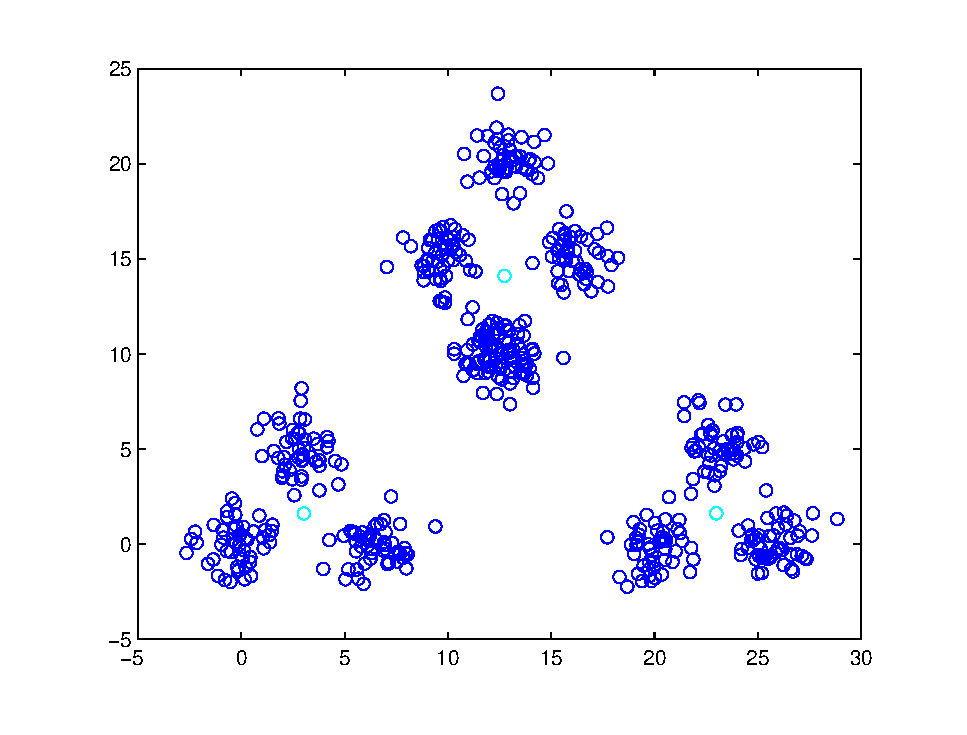
\includegraphics[width=13cm]{Fig/fig_multiple_knee.eps}
 \end{center}
\caption{\small{Data points and found cluster centers with K = 3 in data2 dataset}} 
\label{fig:multipleKnee}
\end{figure}


\section{Feature normalization}

In this section we analyzed the effects of feature normalization and the performance of our K-means clustering algorithm with k = 2 for 200 different random initializations. 
We recorded all the cluster centers that were found in these 200 runs.

\begin{figure}[h]
\begin{center}
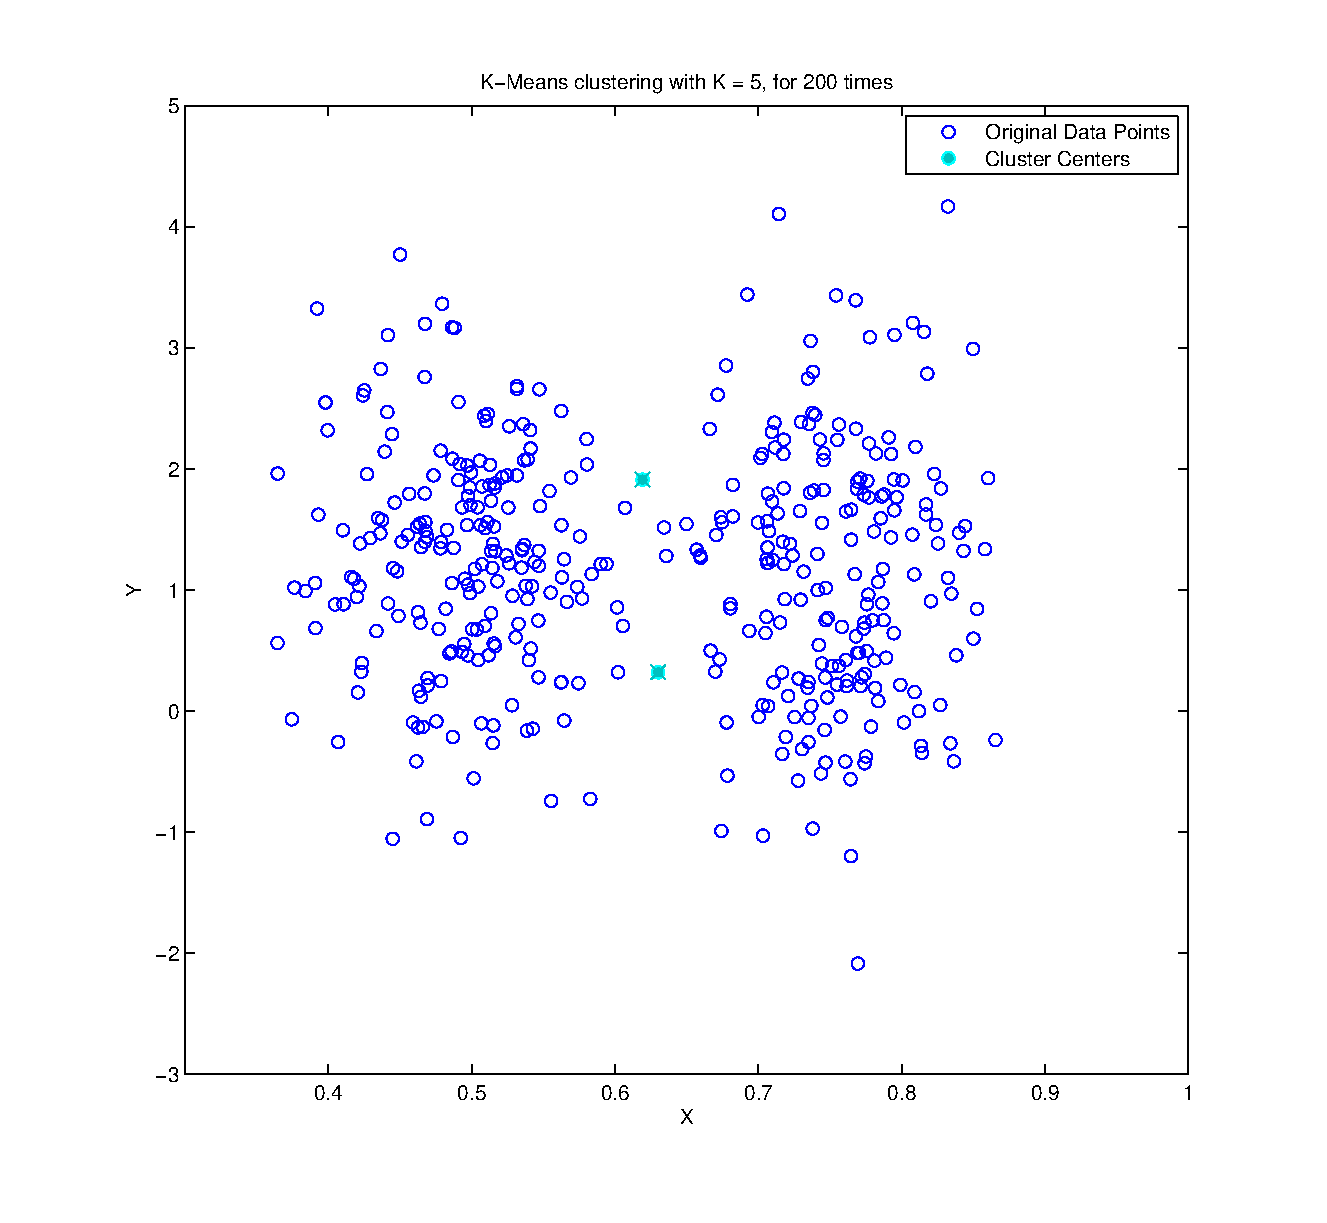
\includegraphics[width=11cm]{Fig/fig_khooboo_3a.eps}
 \end{center}
\caption{\small{K-means clustering over un-normalized data for the data3 dataset with K = 2}}
\label{fig:khooboo_3a_unnormalized}
\begin{center}
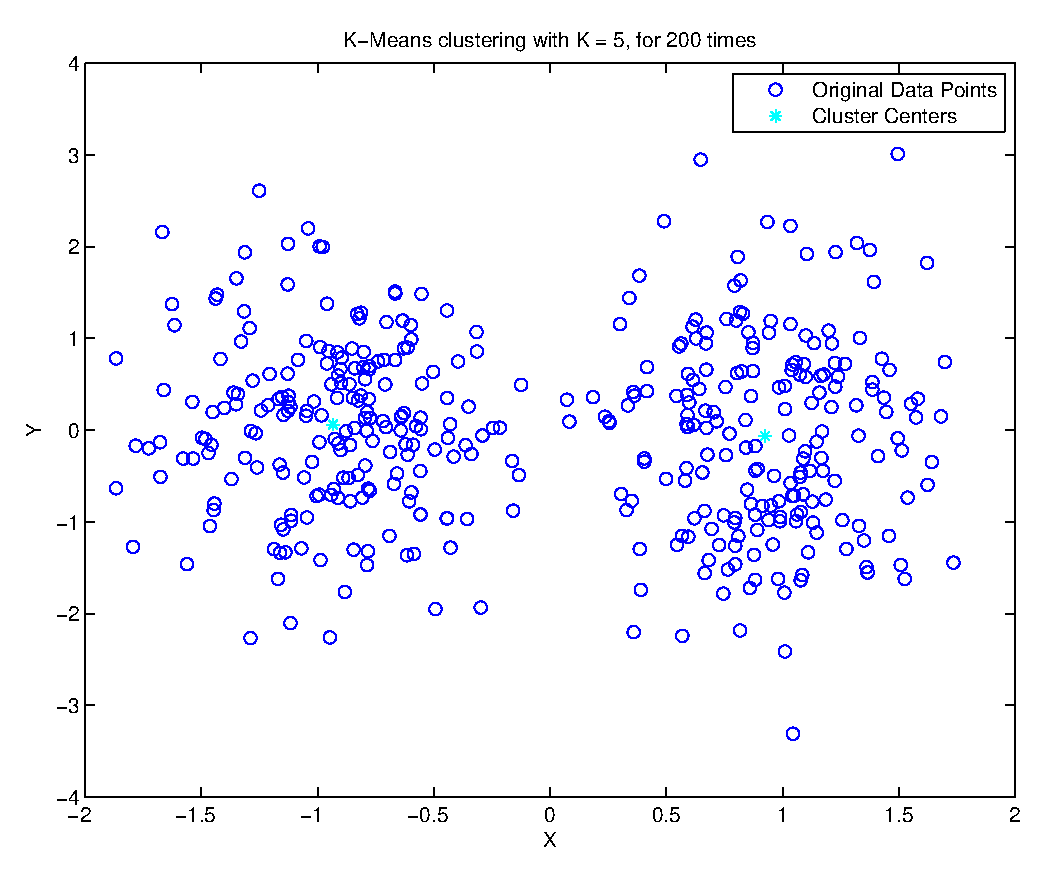
\includegraphics[width=11cm]{Fig/fig_khooboo_3b.eps}
\end{center}
\caption{\small{K-means clustering over normalized data for the data3 dataset with K = 2}} 
\label{fig:khooboo_3b_normalized}
\end{figure}

$Figure~\ref{fig:khooboo_3a_unnormalized}$ shows  the original data in blue color and the cluster centers in the same figure using a cyan color. As seen in this figure, the center of clusters are on the border of two main clusters seen in the figure. 

$Figure~\ref{fig:khooboo_3b_normalized}$ shows the normalized data in blue color and the cluster centers in cyan color. As seen in this figure, the center of clusters are in the center of the two main clusters seen in the figure, which shows that our K-means clustering algorithm performed a better job given normalized data, in case of data3 dataset.  

To normalize the data, we first centered the data to have zero mean(by subtracting the mean from the data), then rescaled each feature dimension to have unit variance. 

%
%\section{Submitted Codes}
%We implemented the  code of this assignment in Matlab language. The submitted codes contains the following files:\\
% 1) $regression_with_l2_regularization_closed_form_sparse_solution.m$: This file contians the code of the linear regression regularization.\\
% 2) $regression_with_l2_regularization_closed_form.m$: This file contians the code of the linear regression regularization with reduced feature vector.\\
% 3) $batch_perceptron.m$: This file contians the code of the preceptron\\
% 4) $voted_perceptron.m$: This file contians the code of the votedPpreceptron\\
%

\end{document}
\bibliographystyle{abbrv}
\footnotesize
\bibliography{nips2012}

